\section{Collision handling with separate chaining}
\subsection{Instruction}
Assume a hash table utilizes an array of 13 elements and that collisions are handled by separate
chaining. Considering the hash function is defined as: h(k)=k mod 13.
\begin{itemize}
\item i) Draw the contents of the table after inserting elements with the following keys:
\begin{center}
\text{32, 147, 265, 195, 207, 180, 21, 16, 189, 202, 91, 94, 162, 75, 37, 77, 81, 48}
\end{center}
\item ii) What is the maximum number of collisions caused by the above insertions?
\end{itemize}

\subsection{Contents of the Hash-table}
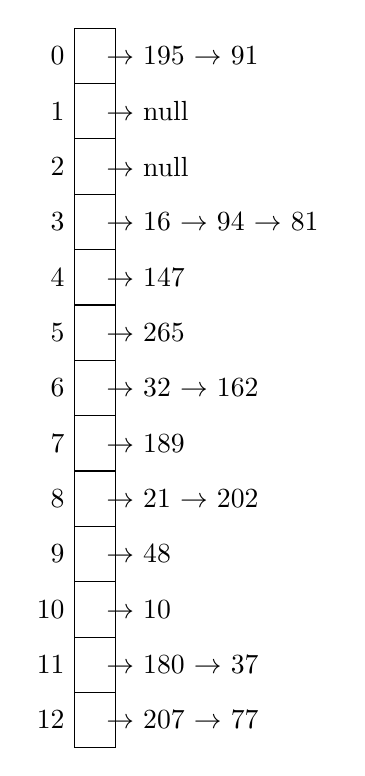
\begin{tikzpicture}
\coordinate (0);
\foreach \t[count=\i from 0,evaluate=\i as\j using int(\i+1)] in {
195 $\rightarrow$ 91  ,
null,
null,
16  $\rightarrow$ 94 $\rightarrow$ 81  ,
147 ,
265 ,
32  $\rightarrow$ 162 ,
189 ,
21  $\rightarrow$ 202 ,
48  ,
10  ,
180 $\rightarrow$ 37  ,
207 $\rightarrow$ 77  
}
\node at(\i.south)[anchor=north,draw,minimum height=2em,minimum width=1.5em,outer sep=0pt](\j){}
    node at(\j.west)[align=right,left]{\i} 
    node at(\j.east)[align=left,right,xshift=-.7em]{$\rightarrow$ \t};
\end{tikzpicture}
\\
\textbf{Contents of the Hash-table after inserting}

\subsection{Maximum number of collisions}
The maximum number of collisions is 3 collisions, happened at index 3 of the table with 3 values 16, 94, 81. The maxim